\documentclass[	11pt, ]{fphw}
\usepackage[utf8]{inputenc} 
\usepackage[T1]{fontenc}
\usepackage{mathpazo}\usepackage{graphicx} 
\usepackage{booktabs} 
\usepackage{listings} 
\usepackage{amsmath}
\usepackage{eso-pic}
\usepackage{array}
\usepackage{float}
\usepackage{graphicx}
\usepackage{bbm}
\usepackage{transparent}
\usepackage{indentfirst}
\usepackage{amsmath,amssymb}
\usepackage{subfigure}
\usepackage{tabu}
\usepackage{enumitem}
\usepackage{caption,tabularx,booktabs}
\usepackage{enumerate} 
\usepackage[english]{varioref}
\renewcommand{\thesection}{\Roman{section}}
\usepackage{titlesec}
\titleformat{\section}
{\normalfont\Large\bfseries}{Exercise~\thesection}{1em}{}
\makeatletter
\renewcommand{\@seccntformat}[1]{
  \csname the#1\endcsname
  \csname suffix@#1\endcsname 
  \quad
}
\renewcommand{\thesubsection}{\alph{subsection}}
\renewcommand{\p@subsection}{\thesubsection.}
% define \suffix@subsection
\newcommand{\suffix@subsection}{)}
\makeatother

\title{Assignment \#8} %
\author{Anita Mezzetti} 
\institute{École polytechnique fédérale de Lausanne} 
\class{Global Business Environment} 
\professor{Luisa Lambertini} 

%--------------------------------------------------------------------
\begin{document}
\maketitle


\section{}
\subsection{}
True. 
\par 
First of all, we tried to understand what means increasing the 'borrowing margin'. A brokerage is an organisation that buys and sells foreign money, shares in companies... for other people. Margin is the money borrowed from a brokerage firm to purchase an investment. It is the difference between the total value of securities held in an investor's account and the loan amount from the broker. Buying on margin is the act of borrowing money to buy securities (tradable financial assets). In other words, buying on margin is the purchase of an asset by using leverage and borrowing the balance from a bank or broker. Buying on margin refers to the initial or down payment made to the broker for the asset being purchased; for example, 20 percent down and 80 percent financed. \\
Regarding mortgage down payment, it is the portion of the total sales price of your home, which you give to the home’s seller. The rest of the payment to the seller comes from your mortgage. Down payments are expressed as percentages. If we buy a house for \$100,000, a 3 percent down payment means that we pay the seller \$3,000 and we borrow \$97,000. \\
If the PBC decides to raise the borrowing margin or the mortgage down payment, people have to pay more. The housing demand will decrease and , consequently, housing prices will deaden. 

\subsection{}
False. 
\par 
A temporary reduction in the money demand has a smaller impact than a permanent one: the long run exchange rate adjusts to the permanent change. So the AA curve shifts out more with a permanent reduction, than a temporary one. If the AA curve shifts out, we have an increase in the exchange rate and an increase in the outputs. Therefore, a permanent reduction has a bigger impact than a temporary one, both in terms of exchange rate and outputs. The formula
\[\Delta Y (1-c+mc)=\alpha \Delta E\]
shows that these two changes are correlated.

\section{}
The economy starts at full employment with an initial CA equals to zero. 
\subsection{}
See figure \vref{aa}: movement from point 1 to 2. \\
The government finances the export subsidity, so the exports increase and consequently the DD curve shifts out. As a result, the AA curve shifts in. This change is permanent so, also in the AA curve, the $E^{e}$ moves. R does not change and Y (considering that we have the same function L) stays put.   \par
This shift in the exchange rate is consistent with the new equilibrium.\\ The fact that the AA curve shifts in makes sense, considering that $\Delta E^{*}<0$. \\We start from Y=C+G+I+CA and we analyse the changes:
\begin{align}
    \Delta Y=&\Delta C+\Delta  G+\Delta I+\Delta CA \\
    \Delta Y=&\Delta C+\Delta CA . 
\end{align}
Considering $C=c(Y-T)$, $CA=\alpha(1+\tau)E-mc(Y-T)$ and the fact that taxes do not change:
\begin{align}
    \Delta Y=&\Delta C+\Delta CA   \\
    \Delta Y=&c \Delta Y+\alpha\Delta E+\alpha \tau E-mc\Delta Y.
\end{align}
We have already stated that $\Delta Y =0$. Then,
\[0=0+\alpha\Delta E+\alpha \tau E-0.\]
Also in this case we conclude that $\Delta E=-E\tau$. 
\par The XX curve moves down. In fact, it shows the combinations of Y and E at which CA is zero. So, in order that $\Delta CA$ stays zero and considering Y does not move (Y=Y' and $\Delta Y=0$) :
\begin{align}
    \Delta CA =& \alpha (1+ \tau )\Delta E  \\
    =& \alpha \Delta E + \alpha E \tau 
\end{align}
If $\Delta CA=0$, then $\Delta E=-E\tau$.


\begin{figure}[h!] 
\centering 
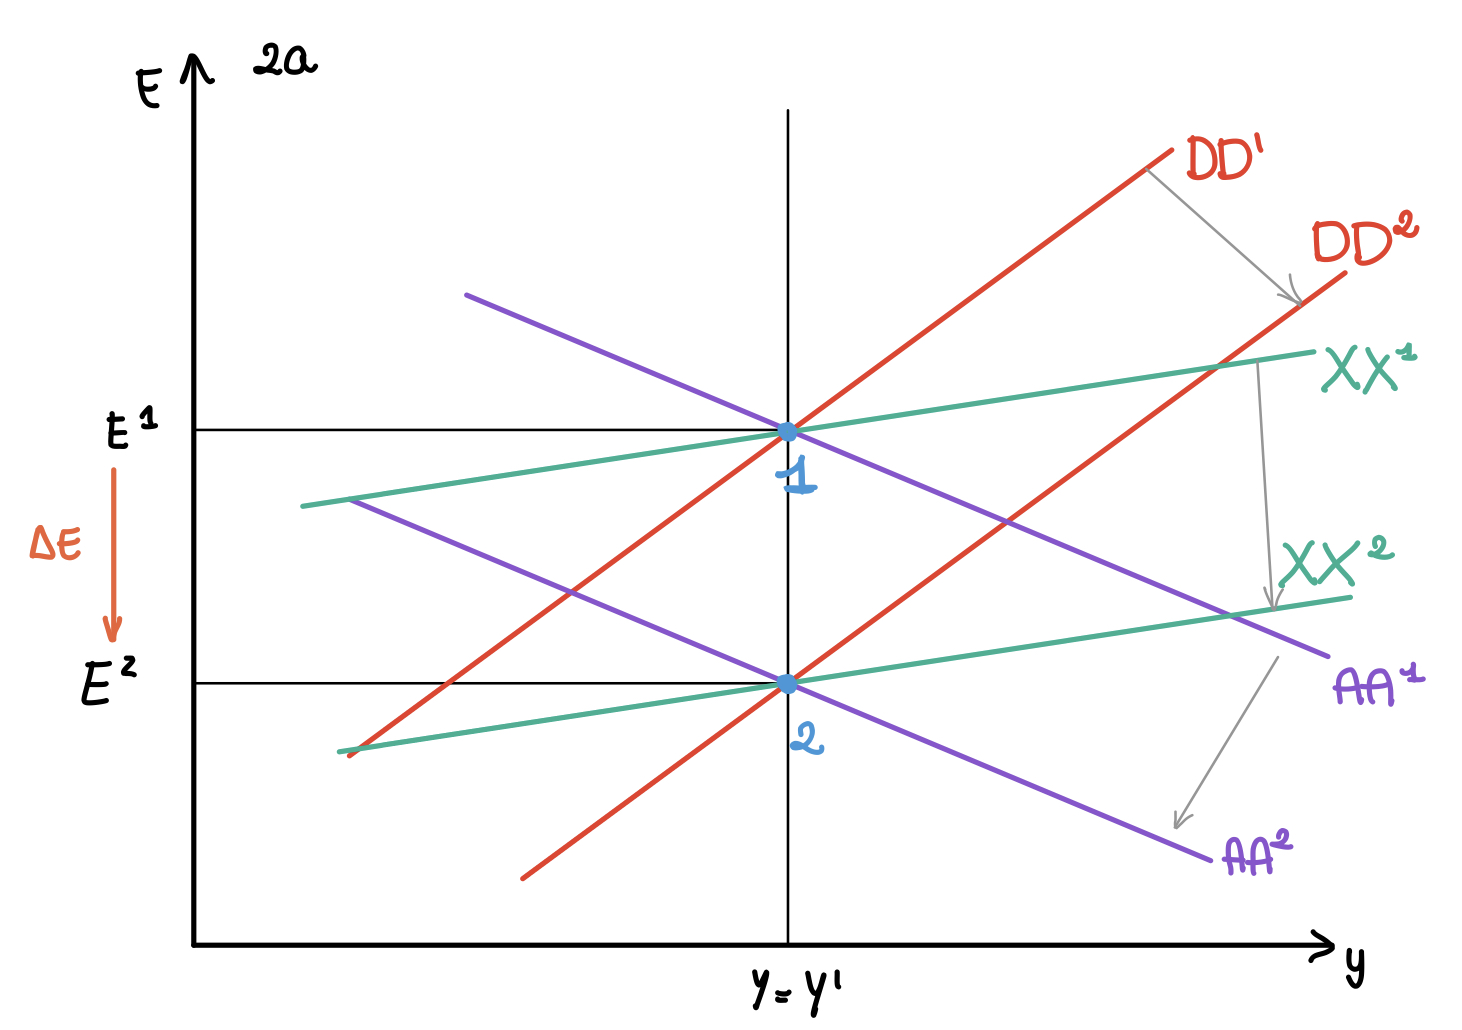
\includegraphics[scale=0.27]{8a.PNG} 
\caption{Question 2.a} 
\label{aa}
\end{figure}

\subsection{}
See figure \vref{bb}. \\
Taxes raise, so $\Delta T >0$. Obviously there will be differences with the previous situation, where we did not consider the contribute of T. In this case the new equilibrium, considering $C=c(Y-T)$, $CA=\alpha(1+\tau)E-mc(Y-T)$ and $\Delta T=\alpha E \tau$, is given by
\begin{align}
    \Delta Y=&\Delta C+\Delta CA   \\
    \Delta Y=&c (\Delta Y-\Delta T)+\alpha\Delta E + \alpha \tau E -mc(\Delta Y-\Delta T). \\
     (1-c+mc)\Delta Y=&c(-1+m)\Delta T +\alpha\Delta E + \alpha \tau E  \\
     (1-c+mc)\Delta Y=&c(-1+m)(\alpha E \tau)+\alpha\Delta E + \alpha \tau E .
\end{align}
Also in this case Y=Y', then
\begin{align}
    0=&c(-1+m)(\alpha E \tau)+\alpha\Delta E + \alpha \tau E  \\
    \Delta E= & (c\tau(1-m)-\tau) E
    \\
    \Delta E= &\tau (c(1-m)-1) E .
\end{align}
Now to understand if $\Delta E$ is positive or negative, we have to analyse c(1-m)-1: $0<m<1$, then $1-m\in (0,1)$; $0<c<1$ and $\tau>0$, then $\tau (c(1-m)-1)<0$. So,
\[\Delta E= - \tau (1-c(1-m)) <0. \]
As in the previous point, the DD curve shifts out. However we have a smaller movement, because the increasing taxes low the demand. Therefore, the AA curve shifts in, always less than the previous point: the movement is partially balanced by the decrease in domestic demand of domestic goods. \\
Going into the current account: 
\begin{align} \label{ca}
    \Delta CA= &\alpha \Delta E + \alpha E \tau +mc \Delta T \\
    =& \alpha \tau c E >0.
\end{align} 
So in this case the equilibrium is not on the XX curve: it is above the line.\\
We have seen that the equilibrium point is not on the XX curve, which moves down. In this case the shift is bigger, in fact the increasing taxes have a positive effect on $\Delta CA$. Due to the fact that the equilibrium point 3 is above the XX curve, this line intersect the output line in a point with a lower exchange rate. If we call $E_{1}$ the exchange rate before the export subsidy and $E_{3}$ the equilibrium exchange rate with also the raising taxes; then we consider $\Delta E$ as the difference of this two. We have calculated it. Instead, $\Delta E^{*}$ will be the difference between $E_{1}$ and the exchange rate where the current account is zero. $\Delta E^{*}$ is 
\begin{align}
\Delta CA = & \alpha \Delta E + \alpha \tau E +mc \Delta T \\
0=&\alpha \Delta E ^{*}+ \alpha \tau E +mc \alpha \tau E \\
0=& \Delta E^{*} + \tau E -mc  \tau E \\
\Delta E^{*} =& \tau (-mc-1) E .
\end{align} 
(-mc-1) is negative, then we switch to -(1+mc) and we observe that 
\begin{align}
    mc>&mc-c  \\
    1+mc>&1-c(1-m).
\end{align}
Then in absolute terms,
\[|\Delta E^{*} | = \tau (1+mc) E> \tau (1-c(1-m))E=|\Delta E|.\]
To explain, we represent the exchange rate movements in the figure.
\begin{figure}[h!] 
\centering 
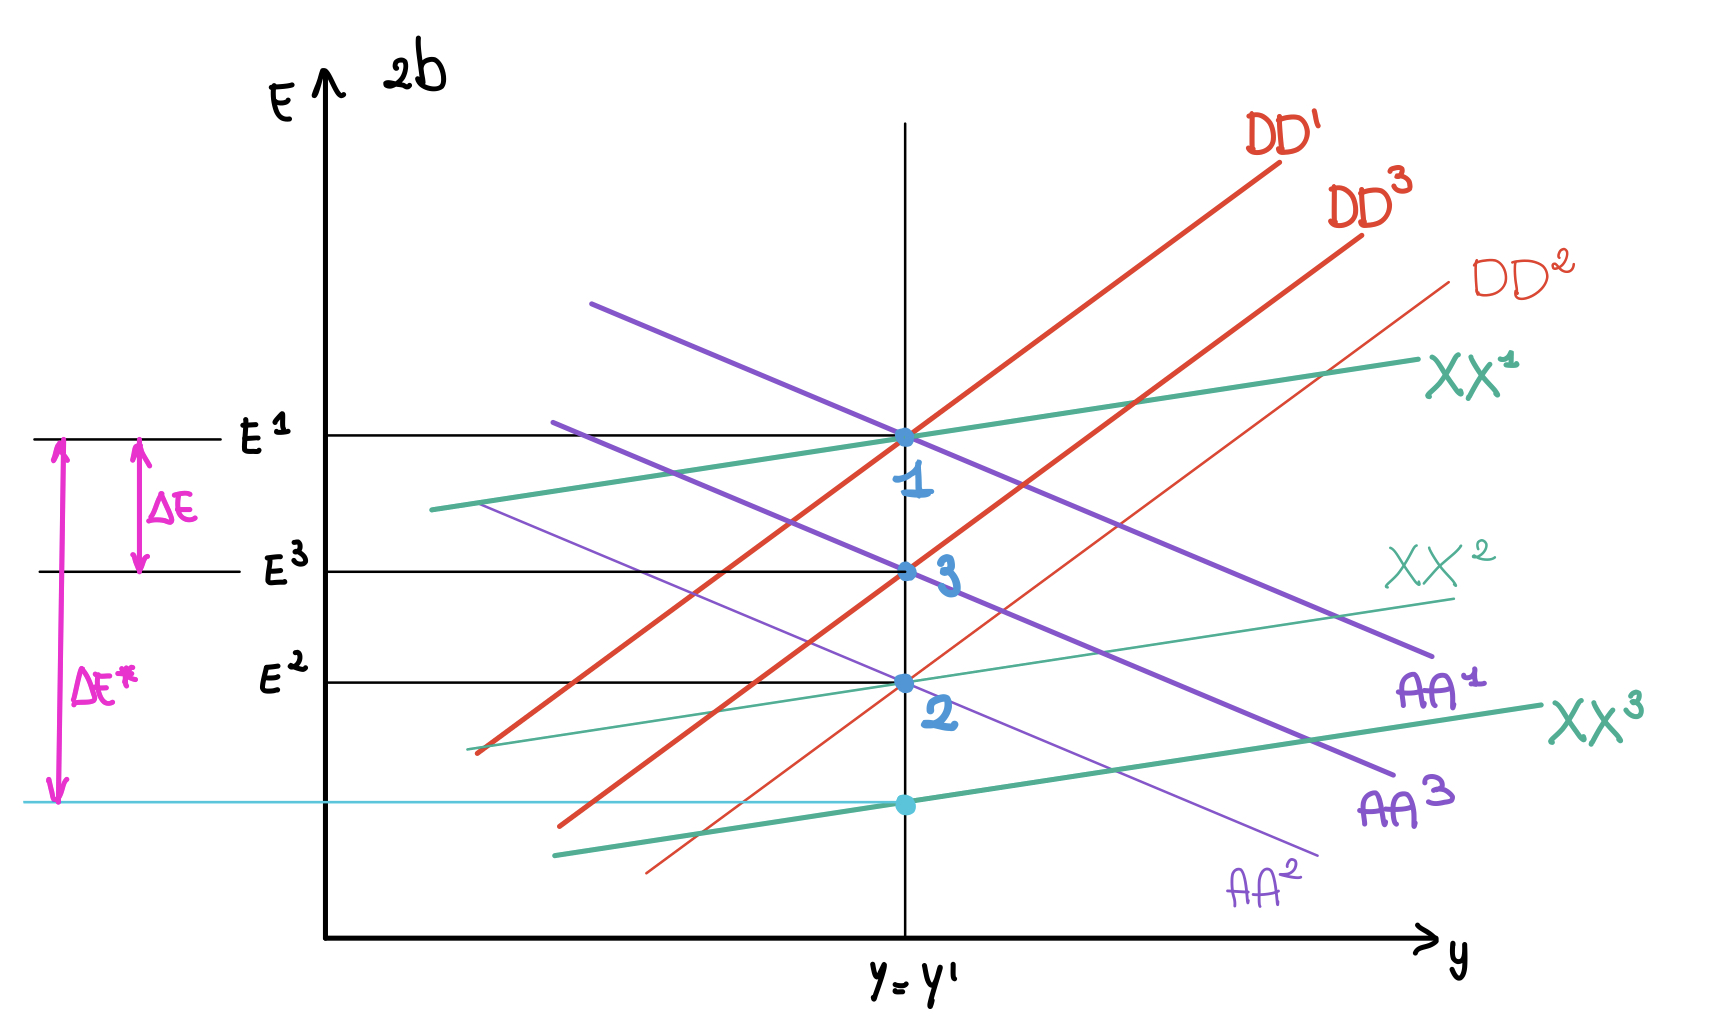
\includegraphics[scale=0.23]{8b.PNG} 
\caption{Question 2.b: the point 2 is the equilibrium point in the question 2.1, while 3 id the equilibrium point in this question} 
\label{bb}
\end{figure}


\subsection{}
See figure \vref{cc}. \\
Now G changes and $\Delta T$ is back to zero:
\begin{align}
    \Delta Y=&\Delta C+\Delta  G+\Delta I+\Delta CA \\
    \Delta Y=&c \Delta Y- \alpha E \tau + \alpha \Delta E + \alpha E \tau -mc\Delta Y  \\
    \Delta Y (1-c+mc)=& \alpha \Delta E
\end{align}
Also in this case Y=Y', then $\Delta E =0$. Therefore the DD curve and the AA curve do not shift. It means that  export subsidy, so the  increase of foreign demand, is completely balanced by a reduction in government spending. The expected exchange rate does not move. \par Regarding the XX curve, we have to study $\Delta CA$:
\[ \Delta CA= \alpha \Delta E + \alpha E \tau = \alpha \tau E.\]
The XX curve shows the points where the current account is zero. If $\Delta CA = 0$, then $\Delta E = -E\tau$.
So, the equilibrium point 4, which is equal to the initial point, is above the XX curve. In particular, the XX line is exactly the same one that we have fount in point 'a' ($XX^{4}=XX^{2}$). 


\begin{figure}[h!] 
\centering 
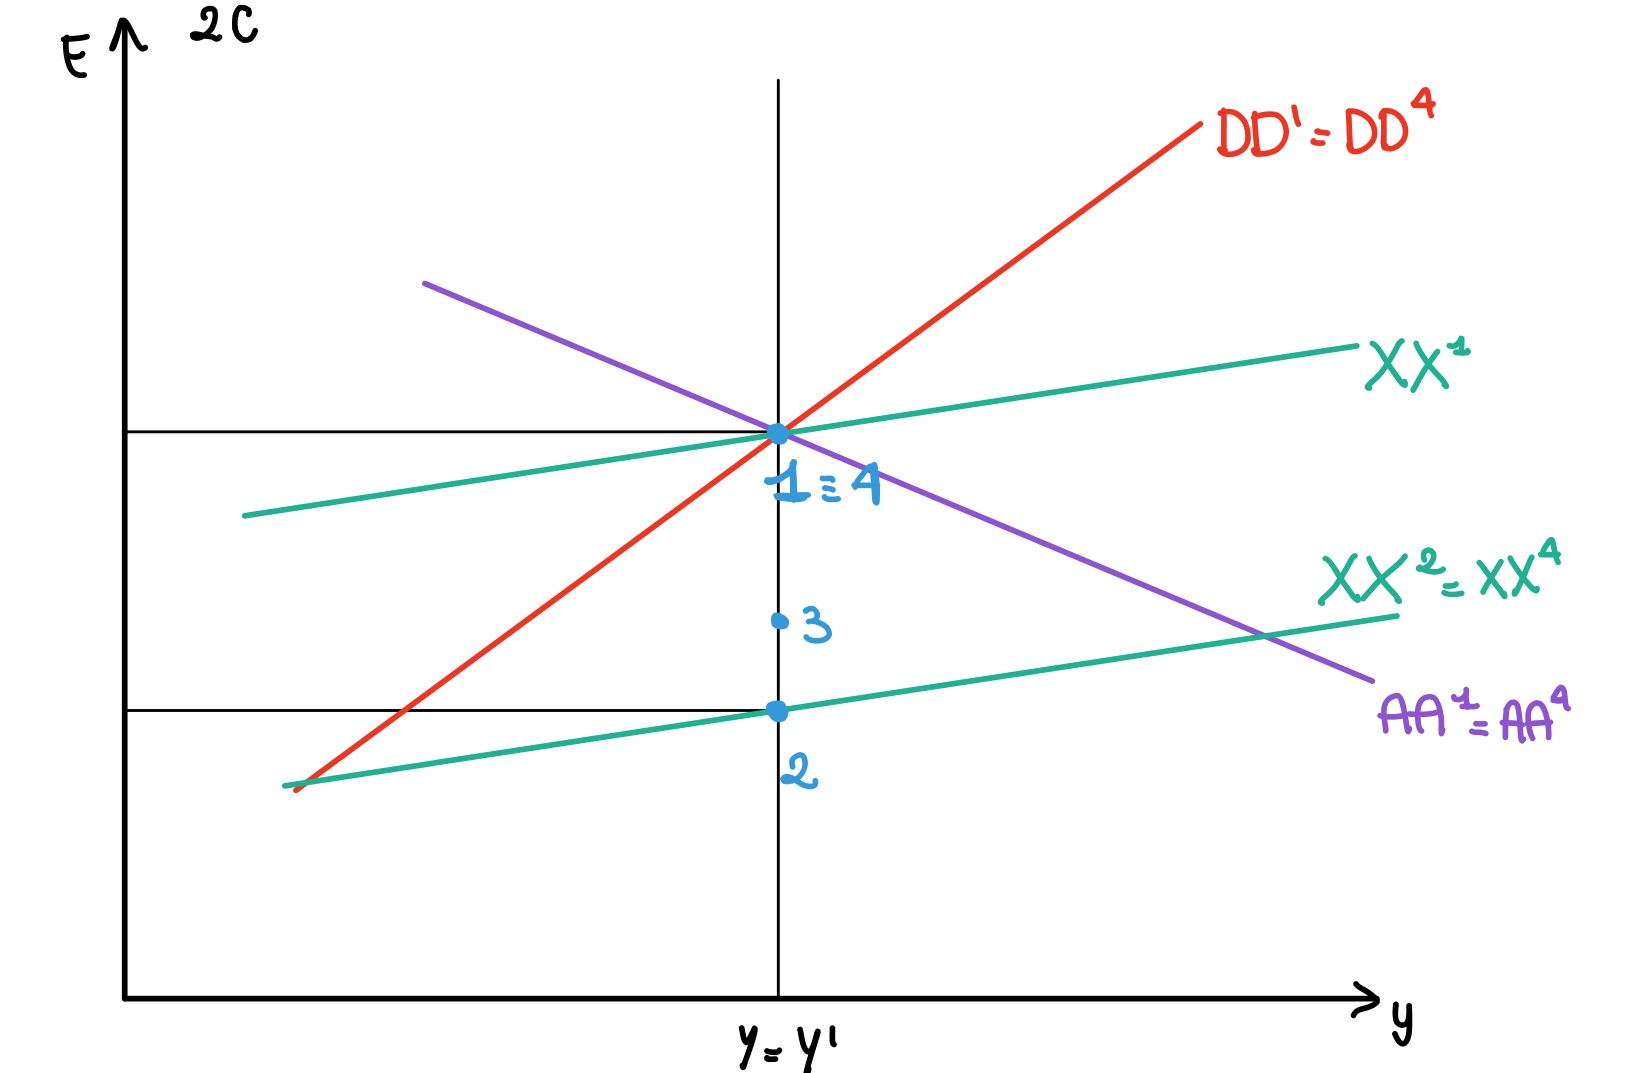
\includegraphics[scale=0.33]{8c.PNG} 
\caption{Question 2.c} 
\label{cc}
\end{figure}

\newpage
\subsection{}
We have seen in the previous questions that, if there is a temporary exports subsidy, the DD shifts out. A temporary change does not have any impact on the expected exchange rate; therefore AA does not shift.
\pat Then the government can act in different ways: if it decrease its spending, this initial change is entirely compensated and the exchange rate do not move. While, if the government decides to increase taxes, the DD curve moves a little inward, but not enough to balance the initial shift outward. In this case the exchange rate shifts: the tax increase does not fully balance the exports subsidy, which leads to an higher domestic demand. The DD curve, which shows the equilibrium points of the output market, shifts out; whereas the AA curve, representing the asset market equilibrium points, stays put.
\par If the government wants to raise output, it want to increase the current account. So it should raise taxes, in order to obtain a positive $\Delta CA$ . This can be done if the XX curve is in the situation of point 'b', where we have shown that the current account is positive (see Equation \ref{ca}). \\
The outputs of new equilibrium point 5 are bigger than the initial ones. 

\begin{figure}[b!] 
\centering 
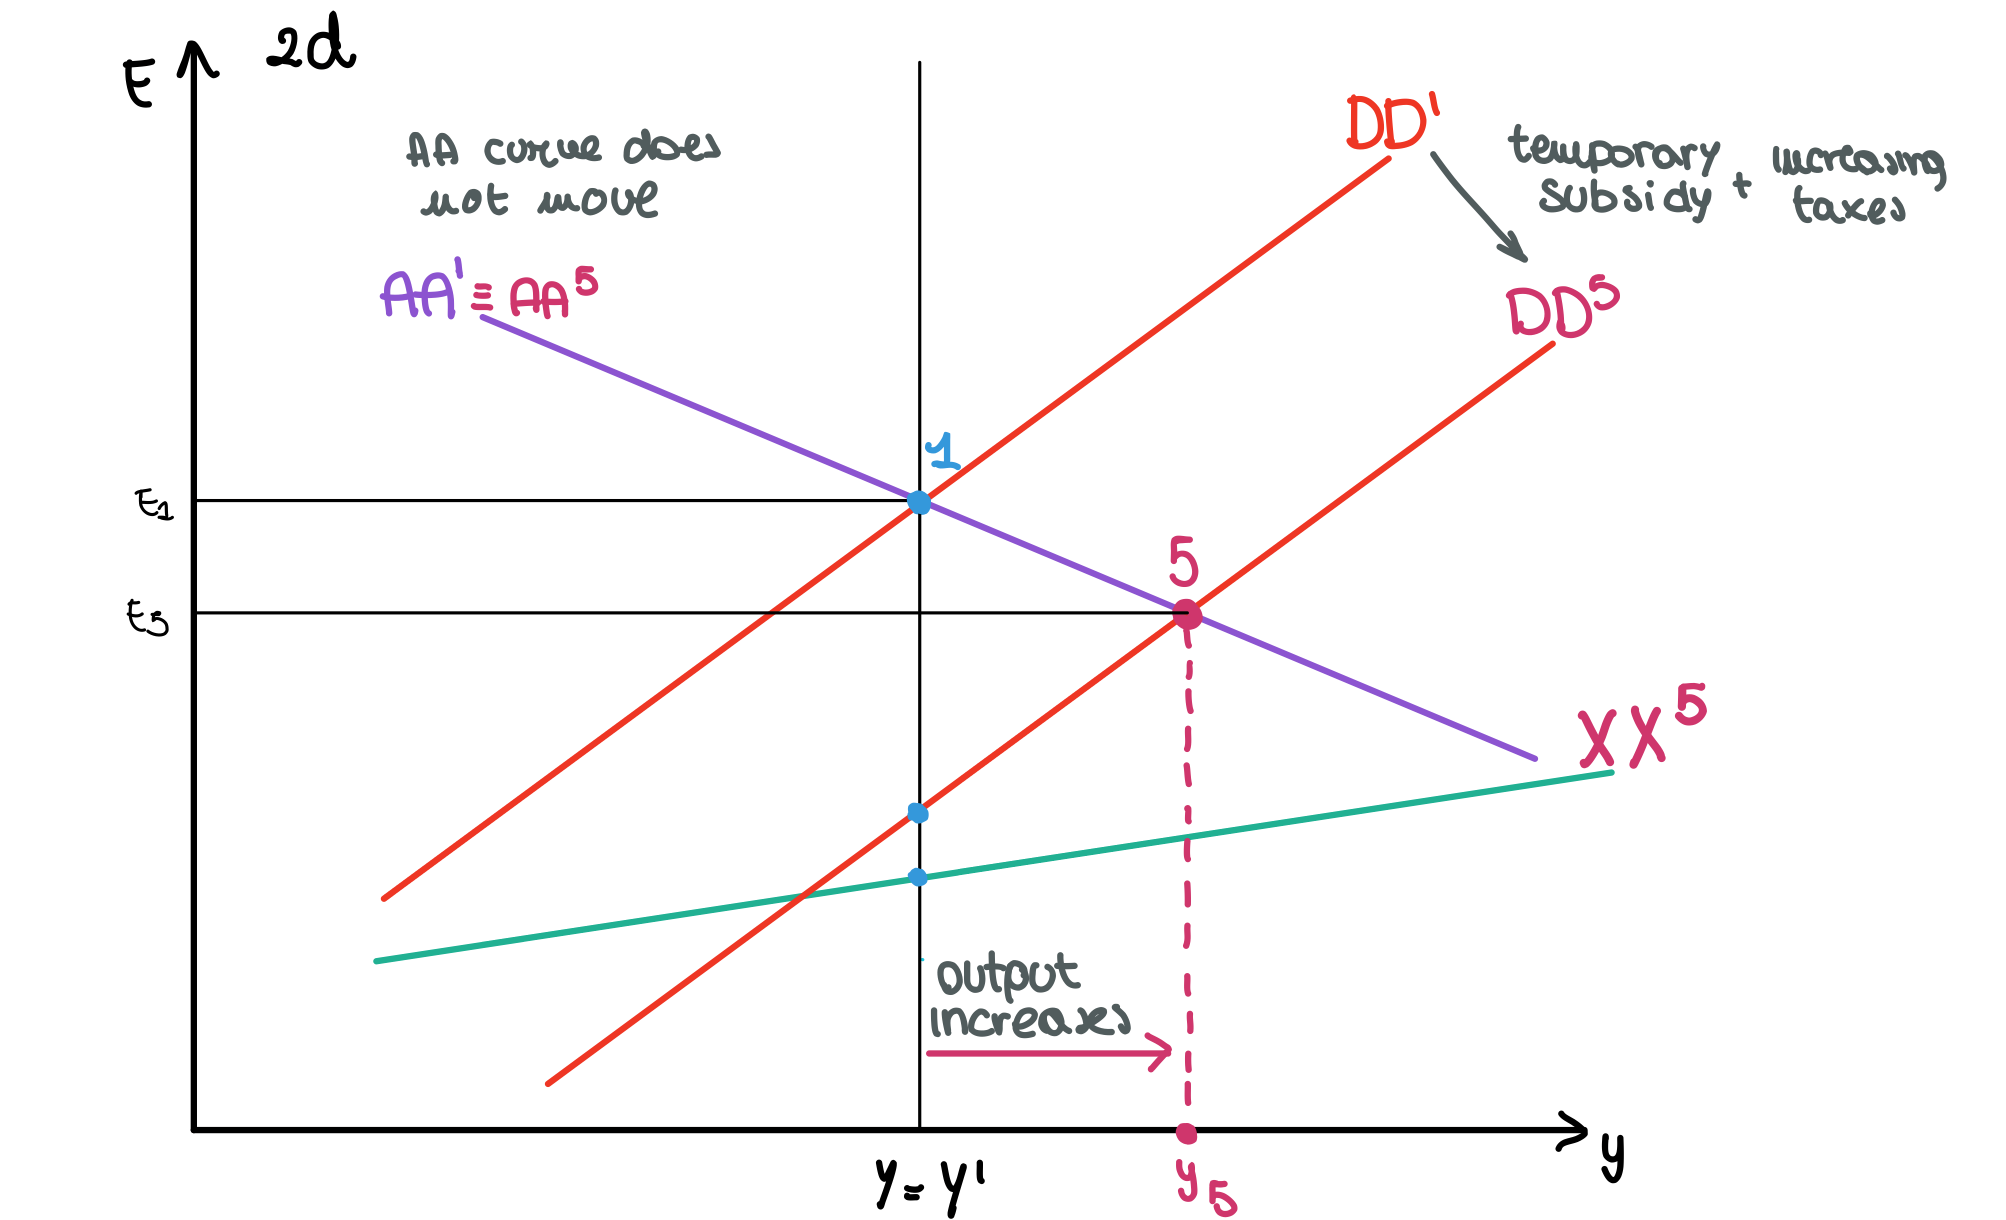
\includegraphics[scale=0.24]{8d.PNG} 
\caption{Question 2.d: temporary subsidy financed by raising taxes} 
\label{dd}
\end{figure}



\end{document}